

\begin{frame}{}
    \centering
    \LARGE
    Toward more expressive update rule: \\the delta rule
\end{frame}

\begin{frame}{Fast weight programming}
    Before diving into the delta rule, let's first review fast weight programming, 
    which will help us understand the delta rule and other test-time-trainers 
    (TTT, Titans, Mesa layer, etc.). 
\begin{tcolorbox}[colback=blue!5,colframe=blue!40,boxrule=0.5pt]
    ``Fast weights provide a neurally plausible way of implementing the type of temporary storage that is required by working memory, while slow weights capture more permanent associations learned over many experiences.''
    \small{ -- Geoffrey Hinton}
\end{tcolorbox}




\vspace{5mm}
%     The hidden state matrix $\mathbf{S}_t$ is a fast weight matrix that is updated at each timestep:
%     \begin{align*}
%         \mathbf{S}_t &= \mathbf{S}_{t-1} + \mathbf{v}_t \mathbf{k}_t^\top
%     \end{align*}
%     \vspace{2mm}

Recall the memory readout in linear attention:
\[
    \mathbf{o}_t = \mathbf{S}_t \mathbf{q}_t
\]
We can think of the recurrent hidden state $\mathbf{S}_t$ as a fast weight matrix that maps input $\mathbf{q}_t$ to output $\mathbf{o}_t$ and is updated as it goes:
\[\mathbf{S}_t = \mathbf{S}_{t-1} + \mathbf{v}_t\mathbf{k}_t^\top\]



\end{frame}



\begin{frame}{Linear attention is secretly a fast weight programmer}
    \resizebox{\linewidth}{!}{
    \begin{tikzpicture}[
        node distance=4.5cm,
        box/.style={
            rectangle,
            draw,
            minimum height=1cm,
            minimum width=1.2cm,
            thick,
            fill=blue!10
        },
        arrow/.style={->,>=latex,thick},
        small box/.style={
            rectangle,
            draw,
            minimum width=0.8cm,
            minimum height=0.8cm,
            inner sep=2pt,
            font=\sffamily,
            fill=orange!10
        },
        values box/.style={
            rectangle,
            draw,
            pattern=north west lines,
            pattern color=green!40,
            fill=green!10,
            minimum size=0.8cm,
            thick
        },
        pink box/.style={
            rectangle,
            draw=pink!80!red,
            thick,
            minimum height=1.2cm,
            minimum width=3cm,
            fill=pink!20,
        },
        weight box/.style={
            rectangle,
            draw=blue!60,
            thick,
            minimum height=1cm,
            minimum width=8cm,
            align=center,
            fill=blue!5
        },
        fast weight box/.style={
            rectangle,
            draw=orange,
            thick,
            fill=orange,
            fill opacity=0.3,
            draw opacity=0.5,
            text opacity=1
        }
    ]
    
    \begin{scope}[on background layer]
        % 状态框
        \node (M1) at (3, 0) {};
        \node[box] (M2) at (4.5,0) {$\mathbf{S}_{t-1}$};
        \node[box] (M3) at (9,0) {$\mathbf{S}_{t}$};
        \node[box] (M4) at (13.5,0) {$\mathbf{S}_{i+1}$};
        
        % Fast weights包裹框
        \path (2.5, 0) -- (M4.south east) node[midway,yshift=-0.5cm] (note) {\small\textbf{\textcolor{orange}{(rapidly changes at each time step)}}};
        \node[fast weight box,fit=(M1)(M2)(M3)(M4)(note),inner sep=10pt] (fastbox) {};
    \end{scope}
    
    % 输入层
    \node[left] at (0.6,6) {\sffamily\Large\bfseries inputs}; 
    \node[box] (X1) at (4.5,6) {$\mathbf{x}_{t-1}$};
    \node[box] (X2) at (9,6) {$\mathbf{x}_t$};
    \node[box] (X3) at (13.5,6) {$\mathbf{x}_{t+1}$};
    
    % Slow weights层
    \node[left] at (0.6,4) {\sffamily\Large\bfseries slow weights};
    \node[weight box] (W) at (9,4) {$\mathbf{W}_q, \mathbf{W}_k, \mathbf{W}_v$\\\small(shared across time steps)};
    
    % 状态间连接
    \draw[arrow] (1.5,0) -- (M2) coordinate[pos=0.95] (M12);
    \draw[arrow] (M2) -- (M3) coordinate[pos=0.95] (M23);
    \draw[arrow] (M3) -- (M4) coordinate[pos=0.95] (M34);
    \draw[arrow] (M4) -- (15.5,0) coordinate[pos=0.95];
    
    % KVQ组
    \foreach \x/\pos/\endpoint/\i/\m in {4.5/a/M12/{t-1}/M2,9/b/M23/t/M3,13.5/c/M34/{t+1}/M4} {
        \node[pink box] (PB\pos) at (\x,2) {};
        \node[small box] (K\pos) at ($(\x,2)+(-0.8,0)$) {$\mathbf{k}_{\i}$};
        \node[small box] (V\pos) at (\x,2) {$\mathbf{v}_{\i}$};
        \node[small box] (Q\pos) at ($(\x,2)+(0.8,0)$) {$\mathbf{q}_{\i}$};
        
        \draw[->,thick] (K\pos.south) to[bend right=45] (\endpoint);
        \draw[->,thick] (V\pos.south) to[bend right=25] (\endpoint);
        \draw[->,thick] (Q\pos.south) to[out=-90,in=90] (\m.north);
    }
    
    % 输入到权重的连接
    \foreach \x in {4.5,9,13.5} {
        \node (X) at (\x,6) {};
        \node (PB) at (\x,2) {};
        \draw[->,thick,blue!60] (X) to[out=-60,in=90] (W);
        \draw[->,thick,blue!60] (W) to[out=-90,in=90] (PB);
    }
    
    % 输出层
    \node[values box] (V2) at (4.5,-2.2) {$\mathbf{o}_{t-1}$};
    \node[values box] (V3) at (9,-2.2) {$\mathbf{o}_{t}$};
    \node[values box] (V4) at (13.5,-2.2) {$\mathbf{o}_{t+1}$};
    
    % 标签
    \node[left] at (0.6,2) {\sffamily\Large\bfseries queries/keys/values};
    \node[left] at (0.6,-2.2) {\sffamily\Large\bfseries outputs};
    \node[left] at (0.6,0) {\sffamily\Large\bfseries fast weights};
    
    % 输出连接
    \draw[arrow] (M2) -- (V2);
    \draw[arrow] (M3) -- (V3);
    \draw[arrow] (M4) -- (V4);
    
    \end{tikzpicture}
    
    }
        
\vspace{-4mm}
\begin{itemize}
    \item {\color{red}\textbf{Fast Weight}}: $\mathbf{S}_t$ maps $\mathbf{q}_t$ to $\mathbf{o}_t$, updated dynamically during inference  for rapid adaptation.
    \item {\color{red}\textbf{Slow Weight}}: $\mathbf{W}_q$, $\mathbf{W}_k$, and $\mathbf{W}_v$ are fixed during inference and only updated during training (e.g., via gradient descent).
\end{itemize}



\end{frame}

\begin{frame}{The choice of update rule}
    \begin{figure}
        \centering
        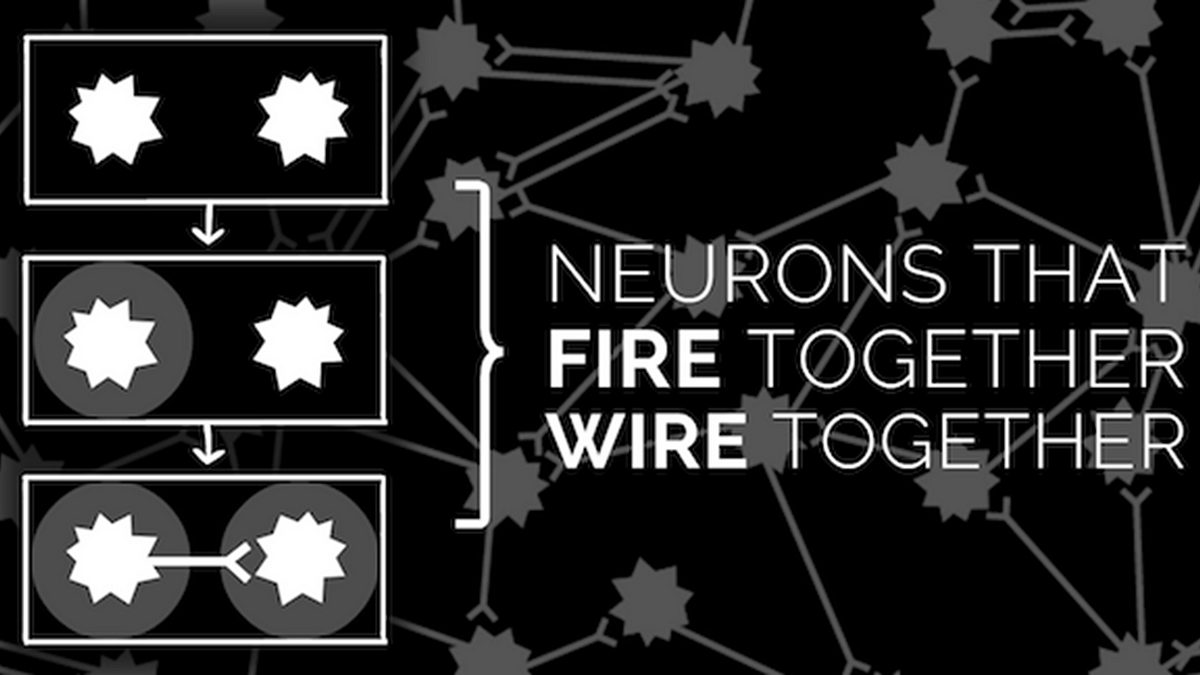
\includegraphics[width=.5\linewidth]{figure/hebbian.png}
        \caption{The principle of Hebbian learning.}
    \end{figure}
    \begin{itemize}
        \item Hebbian update rule: $\mathbf{S}_t = \mathbf{S}_{t-1} + \mathbf{v}_t \mathbf{k}_t^\top$
        \item Delta rule: $\mathbf{S}_t = \mathbf{S}_{t-1} - \beta_t \left(\mathbf{S}_{t-1} \mathbf{k}_t - \mathbf{v}_t\right) \mathbf{k}_t^\top$
        \item ...
    \end{itemize}
    Both Hebbian and delta update rules can be regarded as optimizing online learning objective via {\color{red}test-time SGD}.


\end{frame}
\begin{frame}{Linear Attention: Test-Time Objective}
    \begin{center}
    \begin{tikzpicture}
        \begin{scope}[xshift=3cm]
            \node at (0,3.5) {Maximize alignment};
            \node at (0,3) {= Minimize angle difference + enlarge $|\mathbf{S}\mathbf{k}|$};
            
            \coordinate (O) at (0,0);
            \draw[->,purple,thick] (O) -- (1.75,1.75) coordinate (Mk) node[above] {$\mathbf{S}_{t-1}\mathbf{k}_t$};
            \draw[->,blue,thick] (O) -- (1.5,0.8) coordinate (v) node[right] {$\mathbf{v}_t$};
            
            \draw[->, purple,dashed] (O) -- (3,2.1) node[above] {$\mathbf{S}_{t}\mathbf{k}_t$};
    
            \draw[dashed] (-1,0) -- (2,0);
            \draw[dashed] (0,-1) -- (0,2);
            
            \pic [draw, angle radius=5mm] {angle = v--O--Mk};
        \end{scope}
    \end{tikzpicture}
    \end{center}
\vspace{-2mm}
    \begin{align*}
\hspace*{-1cm}\textbf{Objective: } & \mathcal{L}_t(\mathbf{S}) = -\langle \mathbf{S} \mathbf{k}_t, \mathbf{v}_t \rangle \\[1ex]
\hspace*{-1cm}\textbf{SGD update: } & \mathbf{S}_t = \mathbf{S}_{t-1} - \beta_t \nabla \mathcal{L}_t(\mathbf{S}_{t-1}) = \mathbf{S}_{t-1} + \beta_t \mathbf{v}_t \mathbf{k}_t^\top
    \end{align*}
    \vspace{-6mm}

\end{frame}

\begin{frame}{Linear Attention: Test-Time Objective}
    \begin{center}
        \begin{tikzpicture}
            \begin{scope}[xshift=3cm]
                \node at (0,3.5) {Maximize alignment};
                \node at (0,3) {= Minimize angle difference + enlarge $|\mathbf{S}\mathbf{k}|$};
                
                \coordinate (O) at (0,0);
                \draw[->,purple,thick] (O) -- (1.75,1.75) coordinate (Mk) node[above] {$\mathbf{S}_{t-1}\mathbf{k}_t$};
                \draw[->,blue,thick] (O) -- (1.5,0.8) coordinate (v) node[right] {$\mathbf{v}_t$};
                
                \draw[->, purple,dashed] (O) -- (3,2.1) node[above] {$\mathbf{S}_{t}\mathbf{k}_t$};
        
                \draw[dashed] (-1,0) -- (2,0);
                \draw[dashed] (0,-1) -- (0,2);
                
                \pic [draw, angle radius=5mm] {angle = v--O--Mk};
            \end{scope}
        \end{tikzpicture}
        \end{center}
        \vspace{-4mm}
    \begin{itemize}
        \item Linear attention may favor increasing $|\mathbf{S}\mathbf{k}|$ over angle alignment, leading to numerical instabilities.
        \item Mamba2 uses {\color{red}decay} ($\mathbf{S}_t = {\color{red}\alpha_t} \mathbf{S}_{t-1} + \mathbf{v}_t \mathbf{k}_t^\top$) to control $|\mathbf{S}\mathbf{k}|$, stabilizing the training process.
    \end{itemize}
\end{frame}

\begin{frame}{DeltaNet: Test-Time Objective}
    \begin{center}
        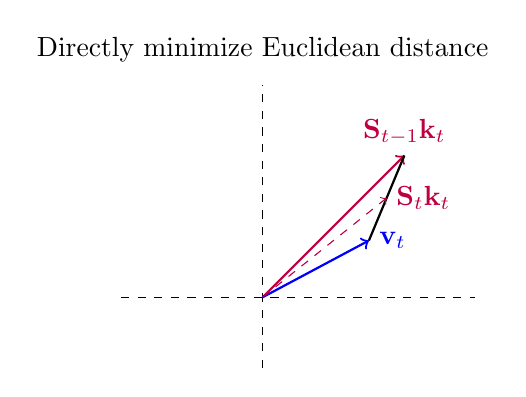
\begin{tikzpicture}[scale=0.9]
            \begin{scope}[xshift=1cm]  
                \node at (0,3.5) {Directly minimize Euclidean distance};
                
                \coordinate (O) at (0,0);
                \draw[dashed] (-2,0) -- (3,0);     
                \draw[dashed] (0,-1) -- (0,3);     
                
                % Original vectors - 调整位置使更分散
                \draw[->,purple,thick] (O) -- (2,2) coordinate (Mk1) node[above] {$\mathbf{S}_{t-1}\mathbf{k}_t$};
                \draw[->,blue,thick] (O) -- (1.5,0.8) coordinate (v) node[right] {$\mathbf{v}_t$};
                
                % Draw the distance line - 需要更新坐标以匹配新的向量位置
                \draw[thick] (2,2) -- (1.5,0.8);
                
                % Dashed vector halfway between Mk1 and v - 调整位置
                \draw[->, purple,dashed] (O) -- (1.75,1.4) node[right] {$\mathbf{S}_{t}\mathbf{k}_t$};
            \end{scope}
        \end{tikzpicture}
     \end{center}
\vspace{-5mm}      
% DeltaNet (\cite{Schlag2021LinearTA, yang2024parallelizing}) optimizes a regression loss via SGD:
    \begin{align*}
        \textbf{Objective: } & \mathcal{L}_t(\mathbf{S}) = \frac{1}{2}\|\mathbf{S} \mathbf{k}_t - \mathbf{v}_t\|^2 \\[1ex]
        \textbf{SGD update: } & \mathbf{S}_t = \mathbf{S}_{t-1} - \beta_t \nabla \mathcal{L}_t(\mathbf{S}_{t-1}) = \mathbf{S}_{t-1} - \beta_t (\mathbf{S}_{t-1} \mathbf{k}_t - \mathbf{v}_t)\mathbf{k}_t^\top 
    \end{align*}
    \vspace{-5mm}

        \begin{itemize}
            \item {\color{red} Better numerical stability}: the norm of $\mathbf{S}_t$ is controlled.
            \item {\color{red} Better in-context associative recall}: directly optimizes key-value association prediction (\cite{Liu2024LonghornSS})
        \end{itemize}
\end{frame}


\begin{frame}{In-context associative recall}
    \begin{block}{\scriptsize Multi-Query Associative Recall (MQAR, \cite{zoology})}
        \scriptsize
        A synthetic benchmark for testing in-context associative recall.
        \vspace{1mm}
        \textbf{Example:}
        \begin{itemize}
            \item Given key-value pairs: ``A 4 B 3 C 6 F 1 E 2''
            \item Query: ``A ? C ? F ? E ? B ?''  
            \item Expected output: ``4, 6, 1, 2, 3''
        \end{itemize}
    \end{block}
    \vspace{-1mm}
    
% \definecolor{color1}{RGB}{145,30,180}
% \definecolor{color2}{RGB}{245,130,48}
% \definecolor{color3}{RGB}{230,25,75}
% \definecolor{color4}{RGB}{123,25,75}
% \definecolor{color5}{RGB}{44,160,44}

\definecolor{color1}{RGB}{116, 184, 22}
\definecolor{color2}{RGB}{77, 171, 247}
\definecolor{color3}{RGB}{99, 230, 190}
\definecolor{color4}{RGB}{132, 94, 247}
\definecolor{color5}{RGB}{250, 176, 5}

\begin{figure}
    \centering
    \resizebox{.5\columnwidth}{!}{  
        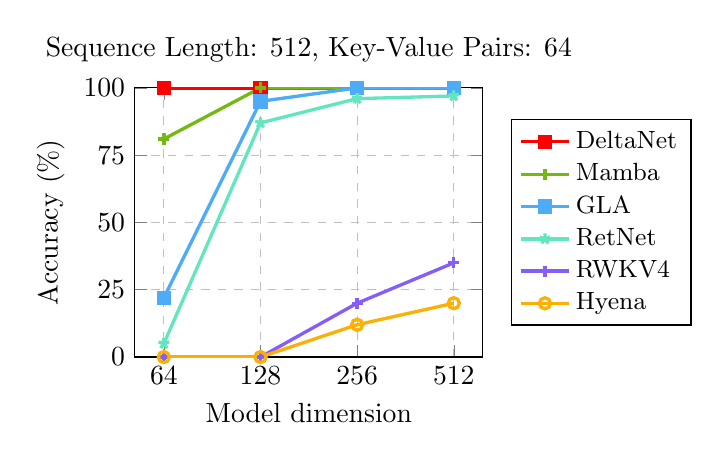
\begin{tikzpicture}
        \begin{axis}[
            name=plot2,
            sharp plot,
            title style={align=right},
            title={Sequence Length: 512, Key-Value Pairs: 64},
            xmode=normal,
            xlabel=Model dimension,
            width=6cm, height=5cm,
            ymin=0, ymax=100,
            symbolic x coords={64,128,256,512},
            ytick={0,25,50,75,100},
            yticklabels={0,25,50,75,100},
            xlabel near ticks,
            ylabel near ticks,
            ylabel=Accuracy (\%),
            ymajorgrids=true,
            xmajorgrids=true,
            grid style=dashed,
            legend style={at={(1.6,0.5)},anchor=east, legend cell align=left, font=\small}, 
        ]

        \addplot[very thick, mark=square*, mark options={scale=1}, color=red] plot coordinates {
            (64,100)
            (128,100)
            (256,100)
            (512,100)
        };
        \addlegendentry{DeltaNet} 

        \addplot[very thick,mark=+,mark options={scale=1}, color=color1] plot coordinates { 
            (64,81)
            (128,100)
            (256,100)
            (512,100)
        };
        \addlegendentry{Mamba} 
        
        \addplot[very thick, mark=square*, mark options={scale=1}, color=color2] plot coordinates {
            (64,22)
            (128,95)
            (256,100)
            (512,100)
        };
        \addlegendentry{GLA} 
        
        \addplot[very thick, mark=star, mark options={scale=1}, color=color3] plot coordinates {
            (64,5)
            (128,87)
            (256,96)
            (512,97)
        };
        \addlegendentry{RetNet}  

        \addplot[very thick, mark=+, mark options={scale=1}, color=color4] plot coordinates {
            (64,0)
            (128,0)
            (256,20)
            (512,35)
        };
        \addlegendentry{RWKV4}  

        \addplot[very thick, mark=o, mark options={scale=1}, color=color5] plot coordinates {
            (64,0)
            (128,0)
            (256,12)
            (512,20)
        };
        \addlegendentry{Hyena} 

        \end{axis}
        \end{tikzpicture}
    }
    \vspace{-3.5mm}
    \caption{Accuracy (\%) on MQAR. DeltaNet achieves the perfect recall.} 
    \label{fig:mqar} 
\end{figure}
\end{frame}


\begin{frame}{Transformers and SSMs in TC$^0$}
    \begin{figure}
        \centering
        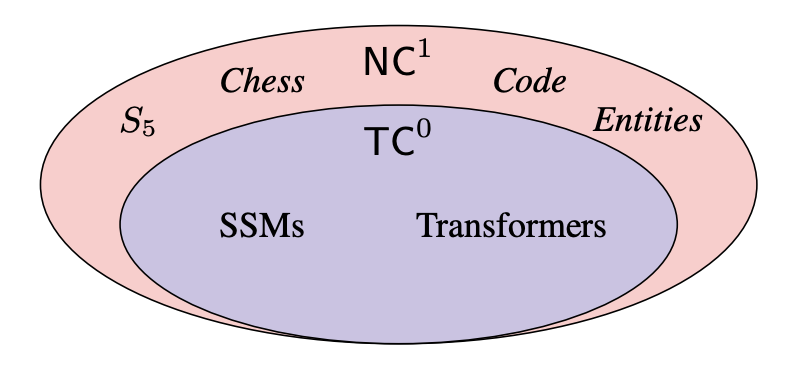
\includegraphics[width=.45\linewidth]{figure/tc0.png}
    \end{figure}
    \vspace{-2mm}
\begin{itemize}
    \item Transformers are in TC$^0$.
    \item Linear RNNs with {\color{red}diagonal transition matrices} (e.g., $\mathbf{S}_t = \mathbf{S}_{t-1} \operatorname{diag}(\boldsymbol{\alpha}_t) + \mathbf{v}_t \mathbf{k}_t^\top$ in GLA) fall under TC$^0$.
    \item {\color{red} Nonlinear RNN} or linear RNN with {\color{red} data-dependent nondiagonal transition matrices} could achieve expressiveness beyond TC$^0$ (\cite{Merrill2024TheIO}).
\end{itemize}
\end{frame}

\begin{frame}{DeltaNet's expressiveness}
    \begin{align*}
    \mathbf{S}_t &= \mathbf{S}_{t-1} - \beta_t \left(\mathbf{S}_{t-1} \mathbf{k}_t - \mathbf{v}_t\right) \mathbf{k}_t^\top \\
    &= \mathbf{S}_{t-1} {\color{blue}\left(\mathbf{I} - \beta_t \mathbf{k}_t \mathbf{k}_t^\top\right)} + \beta_t \mathbf{v}_t \mathbf{k}_t^\top
    \end{align*}

    DeltaNet uses {\color{blue} Generalized Householder} (GH) transition matrices, which are both {\color{red}data-dependent} and {\color{red}nondiagonal}, making it possible to achieve expressiveness beyond $TC^0$.
    % {\color{red}Both conditions} are necessary to achieve expressiveness beyond $TC^0$ (\cite{Merrill2024TheIO}).
\end{frame}



 \begin{frame}{DeltaNet's expressiveness}
    % First show the state update equation
    \begin{align*}
        \mathbf{S}_t &= \mathbf{S}_{t-1} \underbrace{(\mathbf{I} - \beta_t \mathbf{k}_t \mathbf{k}_t^\top)}_{\text{GH transition}} + \beta_t \mathbf{v}_t \mathbf{k}_t^\top 
        = \sum_{i=1}^{t} \left(\beta_i \mathbf{v}_i \mathbf{k}_i^t {\color{blue}\underbrace{\prod_{j=i+1}^{t} (\mathbf{I} - \beta_j \mathbf{k}_j \mathbf{k}_j^\top)}_{\text{cumulative GH products}}}\right)
    \end{align*}

    \vspace{-8mm}
    
    \textbf{Key Properties:}
    \begin{itemize}
        
        \item \textbf{Expressiveness}: When allowing negative eigenvalues in GH matrices (\cite{Grazzi2024UnlockingSI}), {\color{blue}the cumulative products of GH matrices} can represent \textit{any} matrix with Euclidean norm < 1.
        
        \item \textbf{Complexity Class}: 
            {\color{blue}Cumulative products of general matrices} cannot be computed in TC$^0$ (\cite{Mereghetti2000ThresholdCF}).

        \item \textbf{Conclusion}: {\color{red}DeltaNet with negative eigenvalues has expressiveness beyond TC$^0$}, strictly exceeding SSMs and Transformers.
    \end{itemize}
\end{frame}
    

\begin{frame}{State tracking performance}
    \begin{figure}
        \centering
        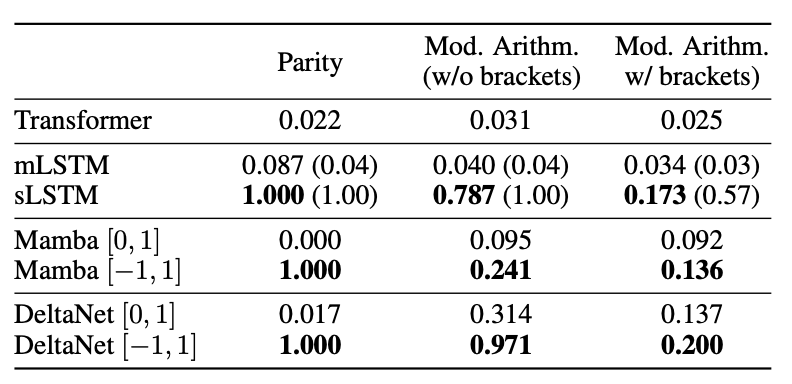
\includegraphics[width=.75\linewidth]{figure/state_tracking.png}
        \caption{State tracking performance comparison (source: \cite{Grazzi2024UnlockingSI}). $[0,1]$ and $[-1,1]$ denotes the ranges of eigenvalues for each model's transition matrix.}
    \end{figure}
    \vspace{-5mm}
   \begin{itemize}
    \item {\color{red}Allowing negative eigenvalues} could boost state tracking performance for both Mamba and DeltaNet.
    \item DeltaNet achieves superior performance due to its {\color{red}richer expressiveness}.
   \end{itemize}
\end{frame}

\begin{frame}{DeltaNet: Chunkwise Parallel Training}
    \begin{align*}
        \mathbf{S}_t &= \mathbf{S}_{t-1} \left(\mathbf{I} - \beta_t \mathbf{k}_t \mathbf{k}_t^\top\right) + \beta_t \mathbf{v}_t \mathbf{k}_t^\top \\
        &= \mathbf{S}_{t-1} + {\color{red}\underbrace{\beta_t(\mathbf{v}_t - \mathbf{S}_{t-1} \mathbf{k}_t)}_{\text{defined as } \mathbf{u}_t}} \mathbf{k}_t^\top \\
        &= \mathbf{S}_{t-1} + {\color{red}\mathbf{u}_t} \mathbf{k}_t^\top \\
        &= \sum_{i=1}^{t} {\color{red}\mathbf{u}_i} \mathbf{k}_i^\top
    \end{align*}    Once ``pseudo-values'' ${\color{red}\mathbf{u}_t}$ are computed, DeltaNet can be trained using the same kernel as linear attention.
\end{frame}


\begin{frame}{DeltaNet: Chunkwise Parallel Training}
    \begin{align*}
        \mathbf{S}_t &= \mathbf{S}_{t-1} \left(\mathbf{I} - \beta_t \mathbf{k}_t \mathbf{k}_t^\top\right) + \beta_t \mathbf{v}_t \mathbf{k}_t^\top \\
        &= \sum_{i=1}^{t} \left(\beta_i \mathbf{v}_i \mathbf{k}_i^\top {\color{blue}\underbrace{\prod_{j=i+1}^{t} (\mathbf{I} - \beta_j \mathbf{k}_j \mathbf{k}_j^\top)}_{\mathbf{P}_j^t}}\right) 
    \end{align*}
    Using the WY representation (\cite{bischof_wy_1985}):
    \[
    \color{blue}\mathbf{P}_{1}^t = \mathbf{I} - \sum_{i=1}^{t}\mathbf{w}_{i}\mathbf{k}_{i}^{\top}.
    \]
    \color{black}
    {\color{red}\textbf{Key Insight}}: The cumulative product $\prod$ becomes a cumulative sum $\sum$, enabling efficient matrix-multiply-based training.
    \end{frame}

\begin{frame}{}
\vspace{-2mm}
    \scalebox{1.0}{
\begin{tikzpicture}
    \foreach \x in {0,5,10,15} {
        \draw[dashed] (\x,-2) -- (\x,2);
    }

        \begin{scope}[shift={(-1.5,0)}]
            \node[draw=black, minimum size=1cm] (grid-0-3) at (0.5,0.5) {};
            \foreach \x in {0,0.33,0.66} {
                \foreach \y in {0,0.33,0.66} {
                    \draw[black] (\x+0.17,\y+0.17) circle (0.12);
                }
            }
        \end{scope}

    \foreach \section [count=\i] in {0.5,5.5} {
        \foreach \offset [count=\j] in {0,1.5} {
            \begin{scope}[shift={(\section+\offset,0)}]
                \node[draw=gray!30, minimum size=1cm] (grid-\i-\j) at (0.5,0.5) {};
                \foreach \x in {0,0.33,0.66} {
                    \foreach \y in {0,0.33,0.66} {
                        \draw[gray!30] (\x+0.17,\y+0.17) circle (0.12);
                    }
                }
            \end{scope}
        }
        
        \begin{scope}[shift={(\section+3,0)}]
            \node[draw=black, minimum size=1cm] (grid-\i-3) at (0.5,0.5) {};
            \foreach \x in {0,0.33,0.66} {
                \foreach \y in {0,0.33,0.66} {
                    \draw[black] (\x+0.17,\y+0.17) circle (0.12);
                }
            }
        \end{scope}
    }
    
    \foreach \section [count=\i] in {0.5,5.5} {
        \begin{scope}[shift={(\section,-1.5)}]
            \foreach \offset [count=\j] in {0,1.5,3} {
                \node[fill=blue!20,draw=black, minimum width=1cm, minimum height=0.4cm] (rect-\i-\j) at (\offset+0.5,0.2) {};
                \foreach \x in {0.2, 0.5, 0.8} {
                    \draw[black] (\offset+\x,0.2) circle (0.1);
                }
                \draw[->,red!30,very thick] (rect-\i-\j.north) to[out=90,in=-90, looseness=0.7] 
                    ([xshift=\j*0cm]grid-\i-3.south);
            }

        \end{scope}
    }
    
\draw[->,yellowgreen,very thick] (grid-0-3.east)  to[bend left=60] (grid-1-3.west);
\draw[->,yellowgreen,very thick] (grid-1-3.east)  to[bend left=60] node[above,xshift=-1.5cm, yshift=0cm,align=center]{
  \textcolor{black}{{\large{\textbf{\color{red}Sequential}} Chunk-Level State Passing:}} 
%   $\color{black}\boldsymbol{S}_{[t+1]}=\boldsymbol{S}_{[t]}
    % {\color{blue!50}\colorbox{yellowgreen!30}{$\mathrlap{({\boldsymbol{I}}-\boldsymbol{W}_{[t]}^\top \boldsymbol{K}_{[t]})}$}} + 
    % {\color{blue!50}\colorbox{red!30}{$\mathrlap{\boldsymbol{U}_{[t]}^\top \boldsymbol{K}_{[t]}}$}}$
} (grid-2-3.west);


\end{tikzpicture}
}

    \vspace{-10mm}
    \begin{align*}
        \boldsymbol{S}_{[t+1]} &= \boldsymbol{S}_{[t]}
        {\color{blue!50}\colorbox{yellowgreen!30}{$\mathbf{({\boldsymbol{I}}-\boldsymbol{W}_{[t]}^\top \boldsymbol{K}_{[t]})}$}} + 
        {\color{blue!50}\colorbox{red!30}{$\mathbf{\boldsymbol{U}_{[t]}^\top \boldsymbol{K}_{[t]}}$}}
    \end{align*}
 Using hardware-friendly UT transform (\cite{Joffrain2006AccumulatingHT}):
    \begin{align*}
        \mathbf{T}_{[t]} &= \left(\mathbf{I} + \operatorname{tril}(\operatorname{diag}(\beta_{[t]})\mathbf{K}_{[t]} \mathbf{K}_{[t]}^\intercal,-1)\right)^{-1}\operatorname{diag}\left(\beta_{[t]}\right) &&\in \mathbb{R}^{C \times C} \\  \mathbf{W}_{[t]} &= \mathbf{T}_{[t]} \mathbf{K}_{[t]}, \quad 
        \mathbf{U}_{[t]}=\mathbf{T}_{[t]}\mathbf{V}_{[t]} && \in \mathbb{R}^{C \times d}
    \end{align*}

    \begin{tcolorbox}[colback=yellowgreen!30,colframe=black,boxrule=0.5pt]
        \footnotesize See \url{https://sustcsonglin.github.io/blog/2024/deltanet-2/} for details.
    \end{tcolorbox}
\end{frame}

\begin{frame}{}
    
\begin{tikzpicture}[
    box/.style={
        rectangle,
        minimum size=0.5cm,
        draw=black!20
    }
]
    \foreach \x in {0,5,10,15} {
        \draw[dashed] (\x,-2) -- (\x,2);
    }
            \begin{scope}[shift={(-1.5,0)}]
            \node[draw=black, minimum size=1cm] (grid-0-3) at (0.5,0.5) {};
            \foreach \x in {0,0.33,0.66} {
                \foreach \y in {0,0.33,0.66} {
                    \draw[black] (\x+0.17,\y+0.17) circle (0.12);
                }
            }
        \end{scope}


    \foreach \section [count=\i] in {0.5,5.5} {

        % \foreach \offset [count=\j] in {0,1.5} {

     \begin{scope}[shift={(\section+1.5,0.1)}]

        \node[box, fill=red!100, minimum size=0.33cm] at (0.17,0.83) {};
        \node[box, minimum size=0.33cm] at (0.5,0.83) {};
        \node[box, minimum size=0.33cm] at (0.83,0.83) {};
        
        \node[box, fill=red!15, minimum size=0.33cm] at (0.17,0.5) {};
        \node[box, fill=red!75, minimum size=0.33cm] at (0.5,0.5) {};
        \node[box, minimum size=0.33cm] at (0.83,0.5) {};
        

        \node[box, fill=red!25, minimum size=0.33cm] at (0.17,0.17) {};
        \node[box, fill=red!45, minimum size=0.33cm] (attn-\i)at (0.5,0.17) {};
        \node[box, fill=red!65, minimum size=0.33cm] at (0.83,0.17) {};
    \end{scope}

        \begin{scope}[shift={(\section+3,0)}]
            \node[draw=black, minimum size=1cm] (grid-\i-3) at (0.5,0.5) {};
            \foreach \x in {0,0.33,0.66} {
                \foreach \y in {0,0.33,0.66} {
                    \draw[black] (\x+0.17,\y+0.17) circle (0.12);
                }
            }
        \end{scope}
    }
    

    \foreach \section [count=\i] in {0.5,5.5} {
        \begin{scope}[shift={(\section,-1.5)}]

            \foreach \offset [count=\j] in {0,1.5,3} {
                \node[draw=black, fill=blue!20, minimum width=1cm, minimum height=0.4cm] (rect-\i-\j) at (\offset+0.5,0.2) {};

                \foreach \x in {0.2, 0.5, 0.8} {
                    \draw[black] (\offset+\x,0.2) circle (0.1);
                }
                \node[draw=black, minimum width=1cm, minimum height=0.4cm,fill=orange!30] (upper-rect-\i-\j) at (\offset+0.5,0.2+3.5) {};
                \foreach \x in {0.2, 0.5, 0.8} {
                    \draw[black] (\offset+\x,0.2+3.5) circle (0.1);
                }
                
            
    \pgfmathsetmacro{\prevsection}{\i-1}
\draw[->, yellowgreen, thick] 
    (grid-\the\numexpr\i-1\relax-3.east) 
    to[bend left=20] 
    (upper-rect-\i-\j.west);

\draw[->, yellowgreen, thick] 
    (rect-\i-\j.north) 
    to[bend left=30] 
    (upper-rect-\i-\j.west);

\draw[->,red!50,very thick] (rect-\i-\j.north) to[out=90,in=-90,looseness=1.2] (attn-\i.south);

\draw[->,red!50,very thick] ([yshift=0.6cm]attn-\i.north) to[out=90,in=-90,looseness=1.2] (upper-rect-\i-\j.south);

}

\ifnum\i>1
\fi

        \end{scope}
    }
    
\node[above=0.25cm,xshift=-3cm,align=center] at (upper-rect-2-2.north) {
  \textcolor{black}{\large{\textbf{\color{red}Parallel} Output Computation:}} \\
%   ${\color{orange}\mathbf{O}_{[i]}}=\colorbox{yellowgreen!30}{${\color{blue!50}\mathbf{Q}_{[i]}}\mathbf{S}_{[i]}^\top$}+\colorbox{red!30}{\color{blue!50}$\left({\mathbf{Q}_{[i]}\mathbf{K}_{[i]}^\top \odot \mathbf{M}}\right)\mathbf{V}_{[i]}$}$
};

\end{tikzpicture}

      \begin{align*}
        {\color{orange}\mathbf{O}_{[t]}} &= \colorbox{yellowgreen!30}{${\color{blue!50}\mathbf{Q}_{[t]}}\mathbf{S}_{[t]}^\top$} + \colorbox{red!30}{$\left({\color{blue!50}\mathbf{Q}_{[t]}\mathbf{K}_{[t]}^\top \odot \mathbf{M}}\right)\left({\color{blue!50}\mathbf{U}_{[t]}}-{\color{blue!50}\mathbf{W_{[t]}}}\mathbf{S_{[t]}^\top} \right)$}
      \end{align*}
      
      Compared to vanilla linear attention, the ``pseudo-values'' need to be adjusted by the historical context: $\mathbf{W}_{[t]}\mathbf{S}_{[t]}^\top$.
\end{frame}



\begin{frame}{Gated DeltaNet}
    Enhancing DeltaNet with a {\color{red}{Mamba2-like gating mechanism}} could boost performance on {\color{red}real-world tasks}.
        \begin{align*}
            \mathbf{S}_t = \mathbf{S}_{t-1} \left({\color{red}\alpha_t}(\mathbf{I} - \beta_t \mathbf{k}_t \mathbf{k}_t^\top)\right) + \beta_t \mathbf{v}_t \mathbf{k}_t^\top
        \end{align*}
    \begin{table}[h!]
        \centering
        \resizebox{0.9\linewidth}{!}{%
            \begin{tabular}{lcccc}
                \toprule
                \textbf{Model} & \textbf{ppl} $\downarrow$ & \textbf{LM-eval} $\uparrow$ & \textbf{Recall} $\uparrow$ & \textbf{Long} $\uparrow$ \\
                \midrule
                Mamba1         & 17.92 & 53.12 & 21.0 & 14.6 \\
                Mamba2         & 16.56 & 54.89 & 29.8 & 13.5 \\
                DeltaNet       & 17.72 & 52.14 & 26.2 & 13.6 \\
                Gated DeltaNet & \textbf{16.42} & \textbf{55.32} & \textbf{30.6} & \textbf{16.6} \\
                \bottomrule
            \end{tabular}
        }
        \caption{Performance comparison of different 1.3B models trained on 100B tokens. Source: \cite{yang2024gateddeltanetworksimproving}.}
        \label{tab:model_comparison}
    \end{table}
\end{frame}
\begin{frame}
    \begin{figure}
        \centering
        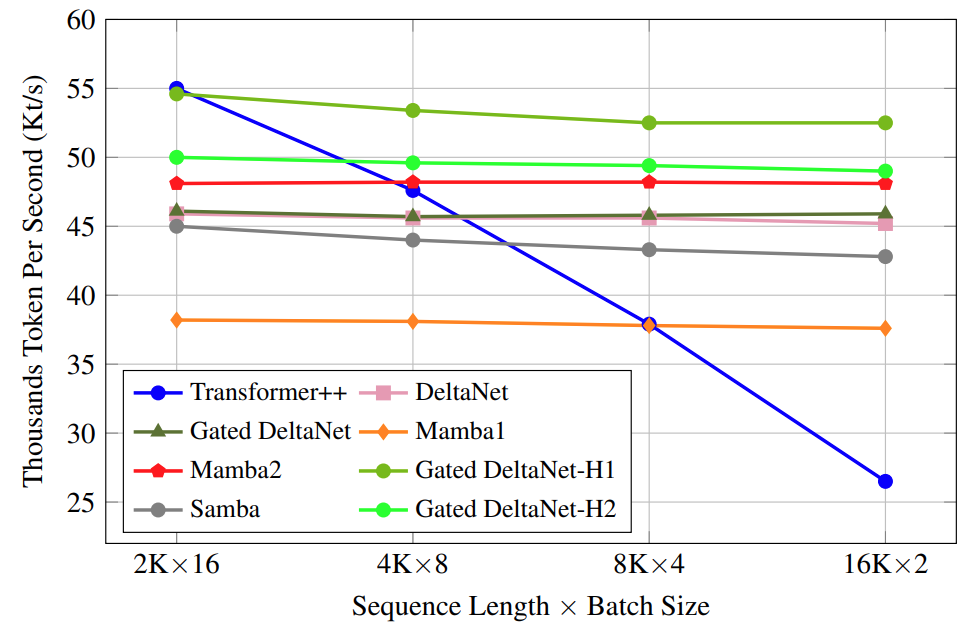
\includegraphics[width=0.65\linewidth]{figure/gdn-speed.png}
        \caption{End-to-end training throughput comparison for different 1.3B models on a single H100. Source: \cite{yang2024gateddeltanetworksimproving}.}
    \end{figure}
    Combining DeltaNet and Mamba2's chunkwise algorithms for hardware-efficient training:
    \begin{itemize}
    \item Pure Gated DeltaNet is slightly slower than Mamba2.  
    \item Hybridizing sliding window attention with Gated DeltaNet (i.e., Gated DeltaNet-H1) improves throughput.
\end{itemize}
\end{frame}

\begin{frame}
    DeltaNet's chunkwise algorithm can be extended to {\color{red}diagonal}-plus-{\color{blue}low-rank} transition matrices:
    \begin{align*}
        \mathbf{S}_t = \mathbf{S}_{t-1} ({\color{red}\mathbf{D}_t} + {\color{blue}\boldsymbol{\alpha}_t \boldsymbol{\beta}_t^\top}) + \mathbf{v}_t \mathbf{k}_t^\top, \quad {\color{red}\mathbf{D}_t \in \mathbb{R}^{d \times d}}, \quad {\color{blue}\boldsymbol{\alpha}_t, \boldsymbol{\beta}_t \in \mathbb{R}^{d}}
    \end{align*}
    \vspace{-5mm}
    \begin{itemize}
        \item \textbf{RWKV-7} employs this linear recurrence, showing effectiveness. 
        \item A fast implementation is available in the flash-linear-attention library (\url{https://github.com/fla-org/flash-linear-attention/blob/main/fla/ops/rwkv7/chunk.py}).
    \end{itemize}
    
    \begin{center}
        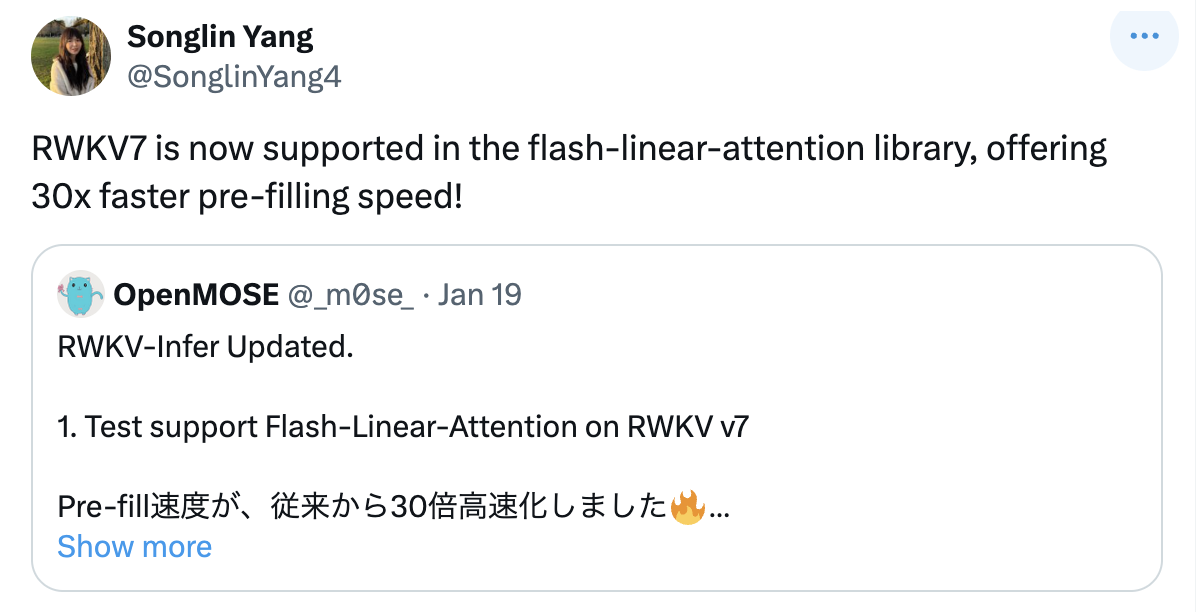
\includegraphics[width=0.75\linewidth]{figure/rwkv7.png}
    \end{center}
\end{frame}

\begin{frame}{DeltaProduct}
    Generalizing the DeltaNet by performing {\color{red}multiple gradient descent steps} (i.e., $n_h$) {\color{blue}per token}:
    \[
    \begin{aligned}
        \mathbf{S}_{{\color{blue}t},{\color{red}j}} &= \mathbf{S}_{{\color{blue}t},{\color{red}j-1}} - \beta_{{\color{blue}t},{\color{red}j}}\nabla\mathcal{L}_{{\color{blue}t},{\color{red}j}}(\mathbf{S}_{{\color{blue}t},{\color{red}j-1}}) \\
        &= \left(\mathbf{I} - \beta_{{\color{blue}t},{\color{red}j}}\mathbf{k}_{{\color{blue}t},{\color{red}j}}\mathbf{k}_{{\color{blue}t},{\color{red}j}}^\top\right)\mathbf{S}_{{\color{blue}t},{\color{red}j-1}} + \beta_{{\color{blue}t},{\color{red}j}}\mathbf{v}_{{\color{blue}t},{\color{red}j}}\mathbf{k}_{{\color{blue}t},{\color{red}j}}^\top
    \end{aligned}
    \]
    where $\mathbf{S}_{{\color{blue}t},{\color{red}0}} = \mathbf{S}_{{\color{blue}t-1}}$ and $\mathbf{S}_{{\color{blue}t},{\color{red}n_h}} = \mathbf{S}_{{\color{blue}t}}$. This results in a \textbf{high-rank} recurrent updates
    \[
    \begin{aligned}
        \mathbf{S}_{\color{blue}t} &= \mathbf{S}_{\color{blue}t-1} \mathbf{A}_{\color{blue}t} + \mathbf{B}_{\color{blue}t} \\
        \mathbf{A}_{\color{blue}t} &= {\color{red}\prod_{j=1}^{n_h}} \left(\mathbf{I} - \beta_{{\color{blue}t}, {\color{red} j}} \mathbf{k}_{{\color{blue}t}, {\color{red} j}} \mathbf{k}_{{\color{blue}t}, {\color{red} j}}^\top\right) \\
        \mathbf{B}_{\color{blue}t} &= {\color{red}\sum_{j=1}^{n_h}} \beta_{{\color{blue}t}, {\color{red} j}} \mathbf{v}_{{\color{blue}t}, {\color{red} j}} \mathbf{k}_{{\color{blue}t}, {\color{red} j}}^\top {\color{red}\prod_{l=1}^{j-1}} \left(\mathbf{I} - \beta_{{\color{blue}t}, {\color{red} l}} \mathbf{k}_{{\color{blue}t}, {\color{red} l}} \mathbf{k}_{{\color{blue}t}, {\color{red} l}}^\top\right)
    \end{aligned}
    \]
    where both the transition matrix $\mathbf{A}_{\color{blue}t}$ and the input $\mathbf{B}_{\color{blue}t}$ are rank-$n_h$ matrices.
\end{frame}

\begin{frame}{DeltaProduct}
    \begin{figure}
        \centering
        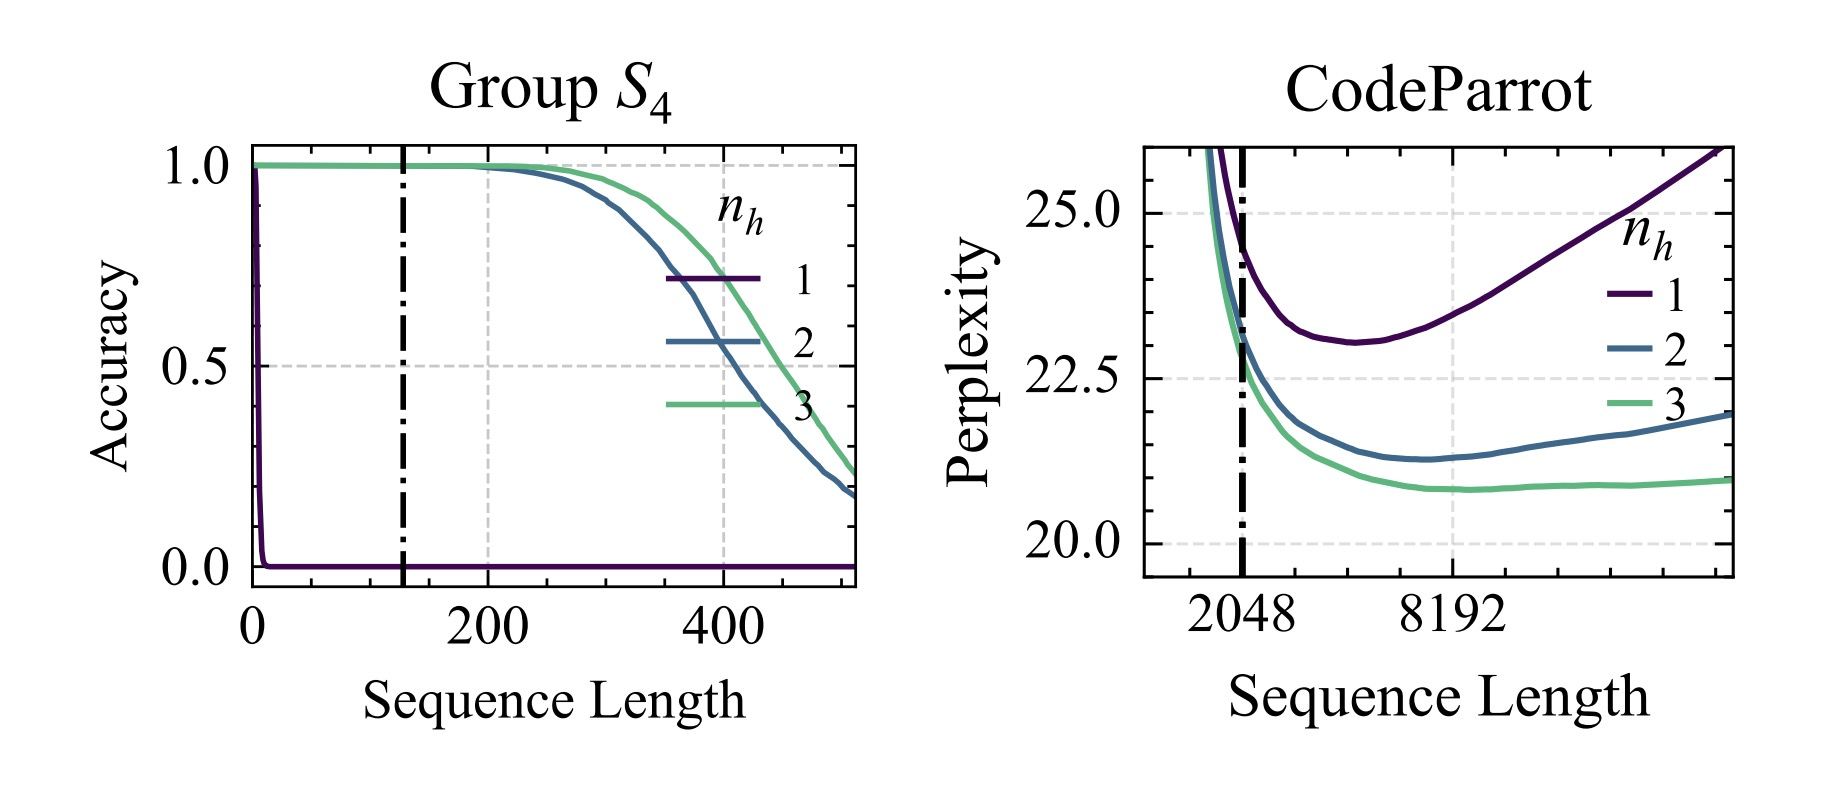
\includegraphics[width=0.9\linewidth]{figure/deltaproduct.jpg}
        \vspace{-4mm}
        \caption{This figure is copied from \cite{siems2025deltaproductincreasingexpressivitydeltanet}.  (\textit{Left}) DeltaProduct$_{n_h}$ learns higher-order permutation groups like $S_4$ in one layer, while DeltaNet ($n_h = 1$) is limited to $S_2$. (\textit{Right}) Length extrapolation of DeltaProduct improves significantly with higher $n_h$.}
    \end{figure}
    
\end{frame}

\begin{frame}{Summary}
    \begin{itemize}
        \item Linear attention and DeltaNet are {\color{red}fast weight programmers} with different {\color{red}test-time SGD} weight updates.
        \item DeltaNet has {\color{red}strictly more expressive power} than Mamba/GLA while {\color{red}maintaining efficient parallelization}
        \item DeltaNet's chunkwise algorithm could be generalized to {\color{red} diagonal-plus-low-rank transition matrices}
        \item {\color{red}Gating} and {\color{red}high-rank updates} further enhance DeltaNet's performance
    \end{itemize}
\end{frame}
